\section{Robot Design}

The robot is powered by four NXT motors at the sides. These are geared up, and
each drive one of the sideways facing holonomic wheels. Holonomic wheels are
used instead of ordinary wheels to allow for smooth on the spot spinning, which
normal wheels are not capable of, as all four do not reside on the same turning
circle. The motors are connected through a spine at the bottom of the robot,
on top of which the solenoid kicker rests, facing forward. The solenoid kicker
does not use a spring to reset itself, and instead relies on the ball being
pushed into it to reset it. The front side of the robot has an old style LEGO
motor on both the left and right sides, each to move a lightweight, slightly
curved grabber arm. Both of these close at the front, and tuck away to the
sides when not used. They are mounted at slightly different heights to allow
them to close fully without colliding.

\begin{figure}[H]
	\begin{center}
    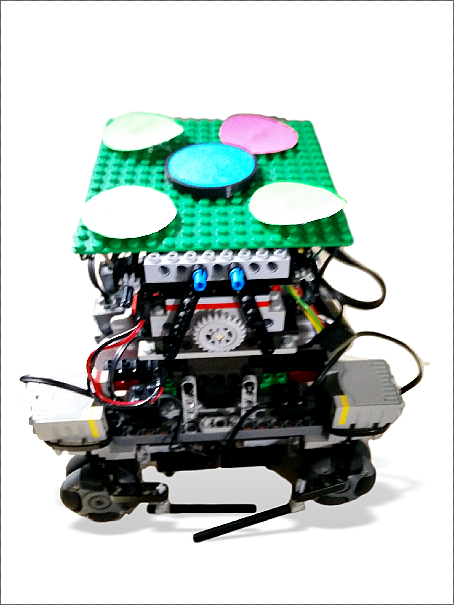
\includegraphics[width=0.35\linewidth]{res/robot.png}
    \caption{Robot}
    \label{fig:goalsandactionsstructure}
	\end{center}
\end{figure}

On the inside of the robot there is some space created by the four movement
motors. This is occupied by a rotary encoder board, which receives input from
the movement motors, the Arduino, along with the supplied motor and power
boards, and various wires and smaller components. These include the wires from
each of the motors, the boards splitting the power and rotary encoder cables
for the NXT motors, and a breadboard regulating the power input for the
solenoid kicker. Both this breadboard, and the power board are wired together,
and both draw power for a battery pack containing 4 lithium-ion batteries
mounted at the rear of the robot. At the base of the battery pack a power
switch is located. A frame is around the loose parts of the robot, and
continues up to the top of the cabling, with beams running above the Arduino to
mount the top plate on.

\section{Hardware Notes}

Grabbing the ball effectively is a fine balance of speed. Moving the grabbers
too quickly kicks the ball away. On the other hand, moving too slowly may lead
to missing the ball. Further, the design of the robot means that the ball must
be pushed in sharply to reset the kicker. The balance between these that was
found, is to close the grabbers at a moderate speed, then rapidly open them
part way and rapidly close them again. This resets the kicker, does not kick
the ball away in most cases, and is fast enough to be usable.

Kicking the ball is a matter of speed, the faster we can kick, the less time
our opponents have to react. However, in order to kick, the ball must also be
positioned precisely in front of the kicker. To achieve this, the grabbers
rapidly push the ball into position again, correcting any drift from movement.
They open part-way, just enough for the kicker to kick without the ball
hitting the grabbers. Finally, the grabbers finish opening.

Spinning and moving tends to move the grabbers about. To avoid this, the
grabbers are powered slightly during both of these actions. If the grabbers are
open, they are constantly opening while the robot is moving, albeit very
slowly. Likewise, the grabbers keep closing if they are already closed. For
this purpose, the robot maintains a local state variable for the grabber. It is
worth stating that this is not measured or sensed, so manually moving the
grabbers will confuse the robot. On startup, the robot assumes the grabbers to
be in their default, open position.
